Quando parliamo di equilibrio chimico omogeneo, con \textit{omogeneo} intendiamo che tutti i composti presenti nella reazione (reagenti e prodotti) sono nella stessa fase, con \textit{equilibrio} intendiamo che a un certo punto si raggiunge una situazione in cui apparentemente non varia più la reazione. Tale situazione è detto di equilibrio.
\subsection{La costante di equilibrio}
\vspace{0.2cm}Facciamo un esempio: consideriamo idrogeno gassoso più iodio gassoso (cosa non naturale per lo iodio in quanto è un solido. Ciò significa che lo abbiamo riscaldato per portarlo in fase vapore):

$$\ce{H_2(g) + I_2(g) <--> 2HI(g)}$$
\vspace{-1cm}\begin{figure}[htp]
    \centering
    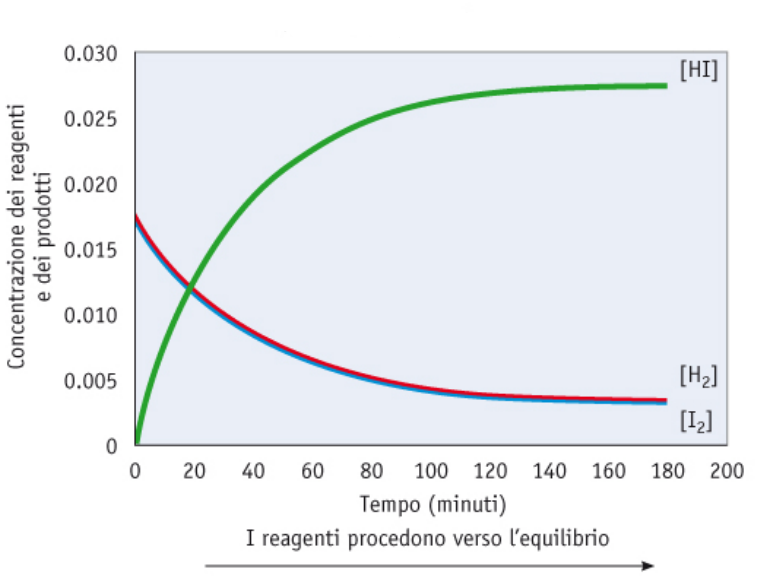
\includegraphics[width=10cm]{immagini/equilibrio_chimico.png}
\end{figure}

Il significato della doppia freccia è che la reazione può procedere in entrambi i sensi: sia da destra verso sinistra che da destra verso sinistra.

I due reagenti considerati danno luogo alla formazione di acido iodidrico, gassoso anch'esso.

L'equilibrio allora è omogeneo perché il prodotto ed entrambi i reagenti sono nella stessa fase.

Il grafico ci mostra che in questa particolare reazione le concentrazioni iniziali dei due reagenti sono uguali (non è necessaria ma conviene), mentre quella iniziale del prodotto è zero, cioè non c'è prodotto al tempo $t=0$.

Appena mescoliamo i reagenti e li facciamo reagire, immediatamente si forma acido iodidrico, ossia la reazione procede da sinistra verso destra.

Nell'istante in cui abbiamo già dell'acido iodidrico formato, piano piano parte la reazione opposta: l'acido si ridissocia per ridare nuovamente i reagenti.

Dato che ciò avviene subito, il processo sarà continuo.

Chiaramente alla fine ci sarà una parte dei reagenti che non ha reagito (o meglio, reagiscono ma poi si ridissociano). Le concentrazioni finali di H$_2$, I$_2$ e HI dipenderanno dalla concentrazioni iniziali di idrogeno e iodio.

\E importante che questa processo avvenga a temperatura fissata.

Si dimostra poi che il rapporto tra la concentrazione (indicata con le parentesi quadre) al quadrato del prodotto HI\footnote{eleviamo perché avevamo coefficiente stechiometrico pari a 2, cioè il coefficiente diventa espondente.} e il prodotto delle concentrazioni dei reagenti (ognuna elevata a 1 perché il loro coefficiente stechiometrico è 1) resta costante nel tempo, ossia è come se non cambiasse per le concentrazioni:

$$\rm \frac{[HI]^2}{[H_2] \cdot [I_2]}=cost$$

In questa fase diciamo che il sistema ha raggiunto l'equilibrio, cioè quando la reazione è in equilibrio tale rapporto non cambia più.

Inoltre possiamo anche partire da concentrazioni diverse tra loro dei reagenti. Ciò che cambierà sarà l'HI finale, ma quel rapporto rimane invariato, a patto che sia mantenuta fissa la temperatura.

Il valore di tale rapporto si chiama \textbf{costante di equilibrio}.

La reazione di ri-dissociazione ha una sua velocità, che è inizialmente diversa dalla reazione di partenza. Da un punto di vista cinetico possiamo dire che abbiamo raggiunto l'equilibrio quando la velocità di trasformazione dei reagenti in prodotto e quella dei prodotti in reagenti si eguagliano. A quel punto si dice che il sistema ha raggiunto l'equilibrio chimico, cioè alla fine le velocità saranno uguali.

Chiaramente anche questo è un equilibrio dinamico, non statico. Ciò significa che le concentrazioni sono fissate, non cambiano, ma ciononostante dell'idrogeno e delle iodio continueranno a reagire per formare dell'acido iodidrico e dell'acido iodidrico si dissocerà per ripristinare idrogeno e iodio in modo continuo. Quindi le reazioni non si fermano, ma non ce ne accorgiamo perché le quantità non cambiano, ssia da un punto di vista delle concentrazioni diciamo che queste sono ormai costanti.

Inoltre in questa reazione non cambia il numero di moli: due moli di reagenti danno due moli di prodotto. Si tratta di un caso particolare, in generale il numero di moli tra reagenti e prodotti varierà.

\vspace{0.2cm}Consideriamo adesso questa reazione:

$$\ce{2NO(g) + 2H_2(g) <--> 2H_2O(g) + N_2(g)}$$

In essa a due moli di ossido di azoto aggiungiamo due moli di idrogeno, per un totale di 4 moli. Tuttavia otteniamo due moli di acqua più una di azoto, per un totale di 3 moli.

Partiamo quindi da 4 moli di 
\subsection{La legge delle masse}

$$\ce{\alpha A + \beta B <--> \gamma C + \delta D}$$

$$\Delta G = RT \ln \frac{P_2}{P_1}, \quad \Delta G= G - G^0$$

$$\Delta G_A = \alpha G_A - \alpha G_A^0 = \alpha RT \ln \frac{P_A}{1}$$

$$\alpha G_A = 0 \implies \alpha G_A = \alpha G_A^0  + \alpha RT \ln P_A$$

Analogamente

$$\beta G_B = \beta G_B^0  + \beta RT \ln P_B,
\quad
\gamma G_C = \gamma G_C^0  + \gamma RT \ln P_C,
\quad
\delta G_D = \delta G_D^0  + \delta RT \ln P_D$$

$$\Delta G_{reazione} = (\gamma G_C + \delta G_D) - (\alpha G_A + \beta G_B)$$

sostituendo

$$\Delta G = (\gamma G_C^0  + \gamma RT \ln P_C + \delta G_D^0  + \delta RT \ln P_D) - 
(\alpha G_A^0  + \alpha RT \ln P_A + \beta G_B^0  + \beta RT \ln P_B)$$

$$\implies \Delta G = \gamma G_C^0 + \delta G_D^0 - \alpha G_A^0 - \beta G_B^0 + RT \ln \frac{P_C^{\gamma} \cdot P_D^{\delta}}{P_A^{\alpha} \cdot P_B^{\beta}}$$

$$\frac{P_C^{\gamma} \cdot P_D^{\delta}}{P_A^{\alpha} \cdot P_B^{\beta}} = k_p
\implies
\Delta G^0 = -RT\ln k_p$$

$$k_p = \frac{P_C^{\gamma} \cdot P_D^{\delta}}{P_A^{\alpha} \cdot P_B^{\beta}}$$

$$PV=nRT \implies P=\frac{n}{V}RT \implies P=c \cdot RT$$

Se indichiamo con [A], [B], [C] e [D] le varie concentrazioni, la $k_p$ sarà

$$k_p = \frac{[\text{C}]^{\gamma} [\text{D}]^{\delta}}{[\text{A}]^{\alpha} [\text{B}]^{\beta}} \cdot \frac{(RT)^{\gamma} (RT)^{\delta}}{(RT)^{\alpha} (RT)^{\beta}}$$

Poniamo

$$k_c = \frac{[\text{C}]^{\gamma} [\text{D}]^{\delta}}{[\text{A}]^{\alpha} [\text{B}]^{\beta}}, \quad \Delta n= (\gamma + \delta - \alpha - \beta)$$

Scriveremo che

$$k_p = k_c \cdot (RT)^{\Delta n}$$


\subsection{Fattori che influenzano l'equilibrio}

\subsubsection{Influenza della pressione}

$$\ce{\alpha A + \beta B <--> \gamma C + \delta D}$$

la costante di equilibrio potrà essere scritta come

$$k_p = \frac{P_C^{\gamma} \cdot P_D^{\delta}}{P_A^{\alpha} \cdot P_B^{\beta}} = \frac{\rchi_C^{\gamma} \cdot \rchi_D^{\delta}}{\rchi_A^{\alpha} \cdot \rchi_B^{\beta}} \cdot P_{tot}^{(\gamma + \delta - \alpha - \beta)}$$

$$\implies k_p = k_{\rchi} \cdot P^{\Delta n}$$
\subsubsection{Influenza della temperatura}